Com a finalidade de validar a interface, foi construído um AV apartir da caracteristicas de um ambiente real(escritório), com planta baixa ilustrada na Figura~\ref{fg:planta_baixa}. Também foram modelados os objetos presentes nessa cenário real, como : computadores, monitores, bancadas, divisórias de vidro e porta.\\

\begin{figure}[ht!]
	\centering
	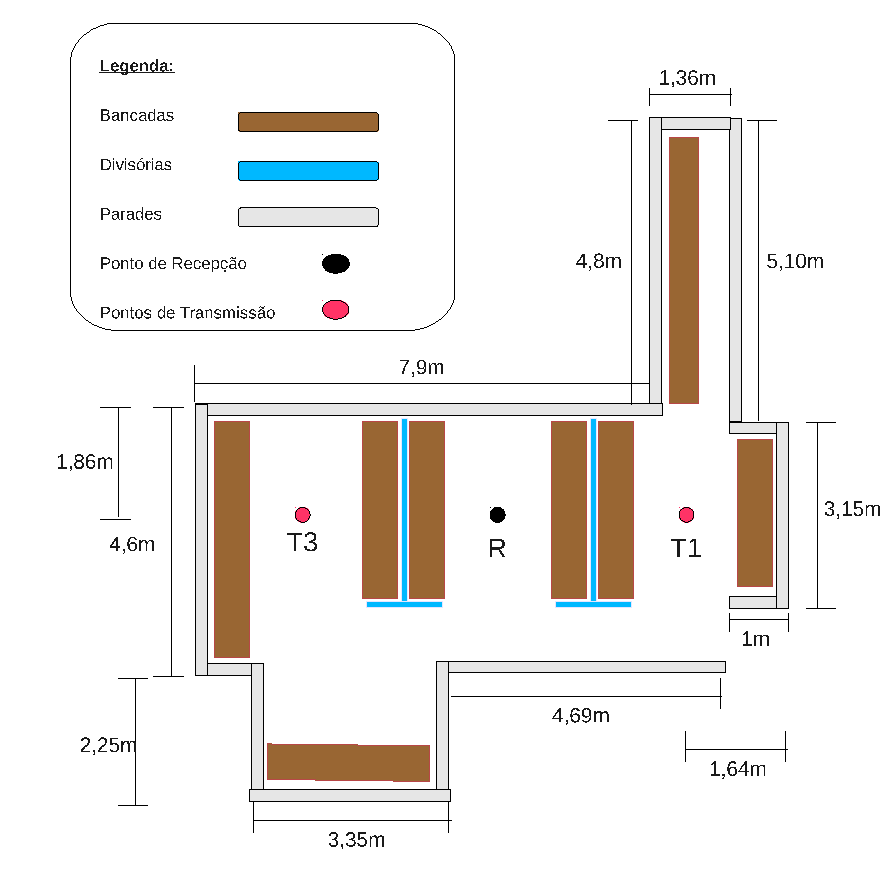
\includegraphics[scale = 1]{planta_baixa}
	\caption{Planta baixa do escritório modelado usando a interface.}
	\label{fg:planta_baixa}
\end{figure}

Esperimentalmente, posde-se observar o comportamento da propragação do sinal de uma antena nesse escritório. 

Alguns desse objetos estão dispostos em alturas diferentes em relação ao piso. As bancadas e o teto estão a uma altura de 0,75 metros e 2,73 metros, respectivamente.\\

Como resultado da modelagem usando a interface, obeteve-se a estrutura mostrada na Figura(colocar figura estrutura da interface). A disposição dos seus objetos seguiu a posicionamento real dos mesmos no momento das medições.
%\begin{figure}[ht!]
%	\centering
%	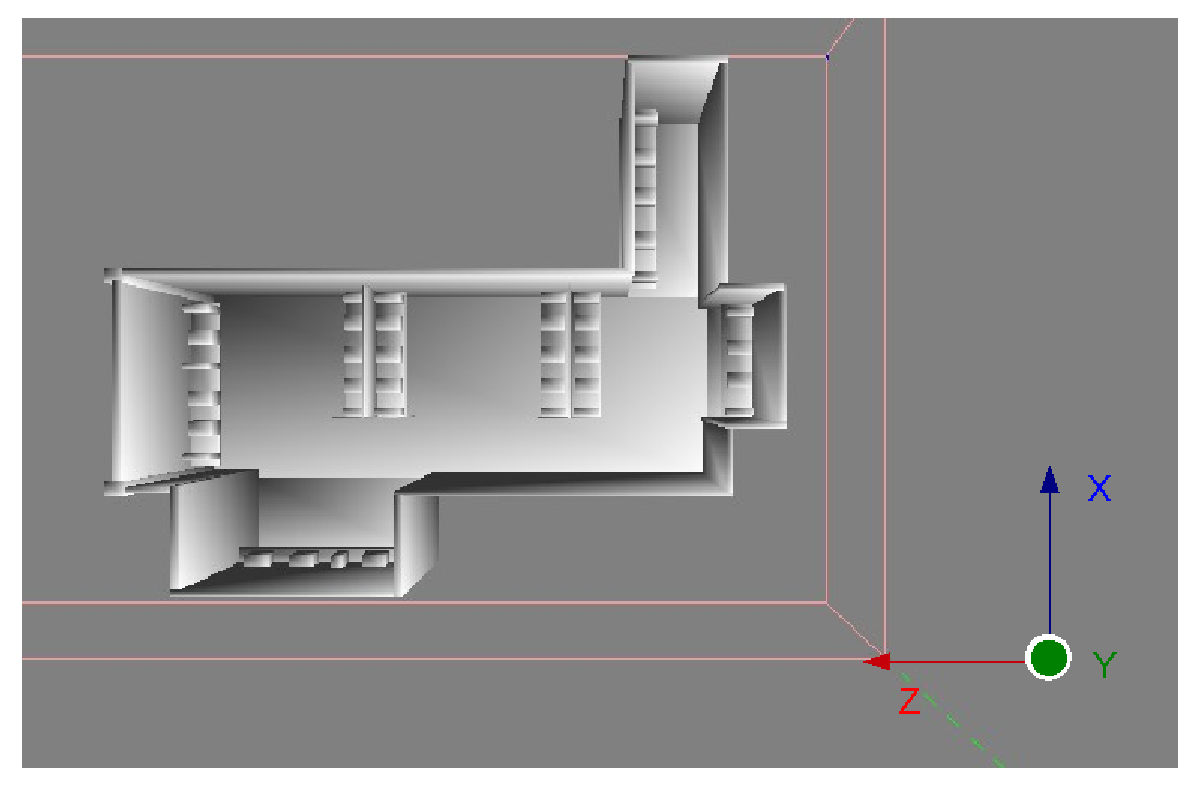
\includegraphics[scale = 0.4]{ambiente}
%	\caption{Visão topo em pespectiva do ambiente construído através da interface.}
%	\label{fg:ambiente}
%\end{figure}

As especificações desse cenário, foram:
\begin{itemize}
\item \textit{Delta}(Tamanho da célula de Yee) utilizada foi de $0,003m$.
\item \textit{Região de Análise} com dimensões: $X$ = $15m$, $Y$ = $3m$ e $Z$ = $15m$.
\item \textit A lista das carateristicas físicas com seus respectivos matérias estam presentes na Tabela~\ref{tab:materiais}
\end{itemize}

\begin{center}
	\begin{tabular}{|l|l|l|l|l|}
	\hline
	Elementos dos Ambiente & Material & $\epsilon$ & $\sigma$ & $\mu$ \\ \hline
	Parede & Tijolo & 4 & 0,0135 & 1\\ \hline
	Teto & Gesso & 2,8 & 0,1533 & 1 \\ \hline
	Bancadas & Madeira & 1,8 & 0,011 & 1\\ \hline
	Monitores e Gabinetes & Metal & 5 & $valor$ & 1\\ \hline
	Divisórias & Vidro & 5 & $valor$ & 1 \\ \hline
	Piso & Concreto & 5 & 1 & 1 \\
	\hline
	\end{tabular}
	\label{tab:materiais}
\end{center}

%antena
Depois de ambiente ter sido montado, surguiu a necessidade de se introduzir a antena . Como a que foi usada na medição não tinha uma representação virtual, foi necessário criá-la. Com isso foram feitos alguns teste usando antenas dipolo, com o intuito de obeter a máxima aproximação do comportamento da antena real. \\

Para todos os modelos de antena foi ultizada uma fonte de tensão de trêm de pulsos normalizado, Figura~\ref{fg:fonte}, onde através da transforma de Fourier, pode-se observar se a mesma estava trabalhando na banda adequada. O resultado obtido foi o ilustrado na Figura~\ref{fg:fonte_f}.\\

A primeira antena feita foi um dipolo mostrado na figura~\ref{fg:antena_normal}

%\begin{figure}[ht!]
%	\centering
%	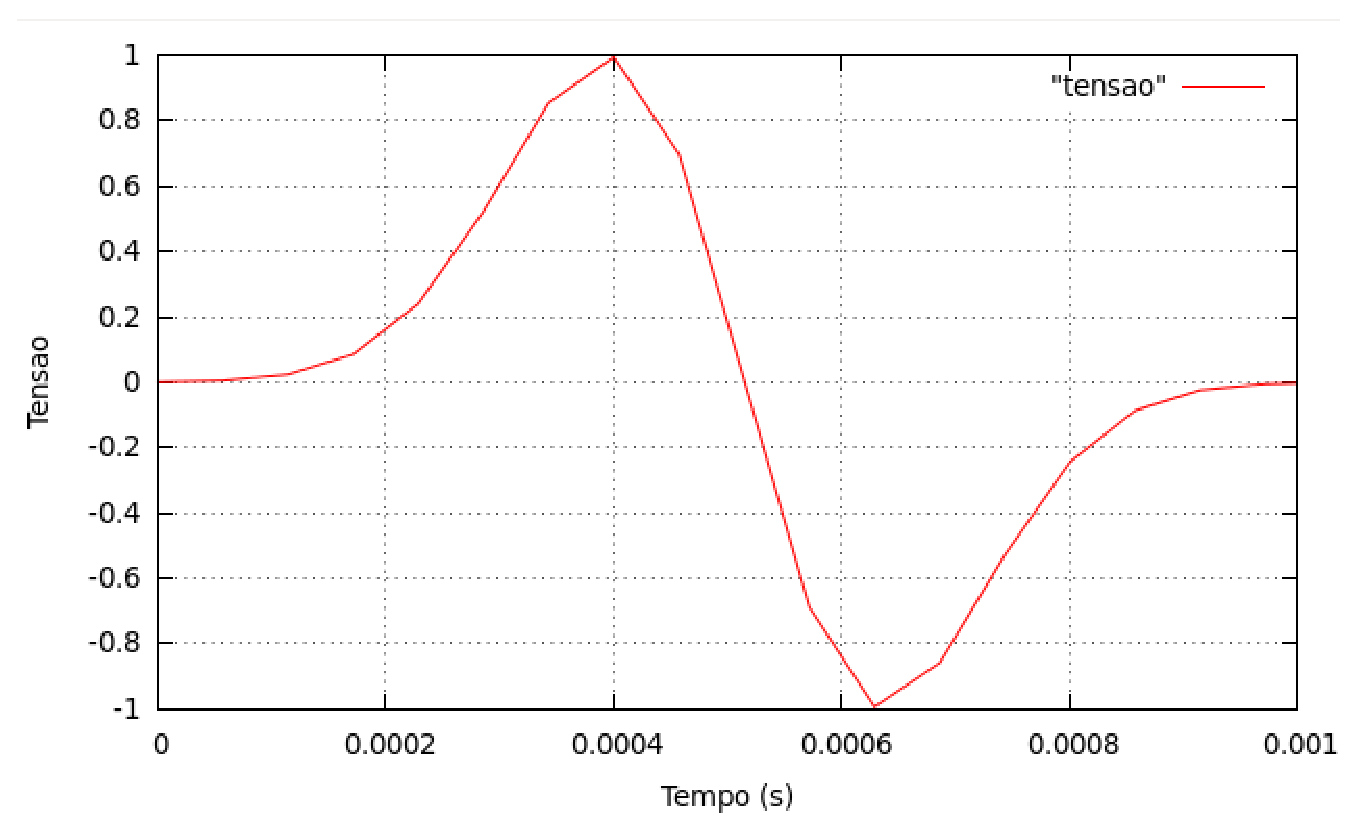
\includegraphics[scale = 0.4]{tensao}
%	\caption{Gráfico da fonte(trêm de pulsos).}
%	\label{fg:fonte}
%\end{figure}
%\begin{figure}[ht!]
%	\centering
%	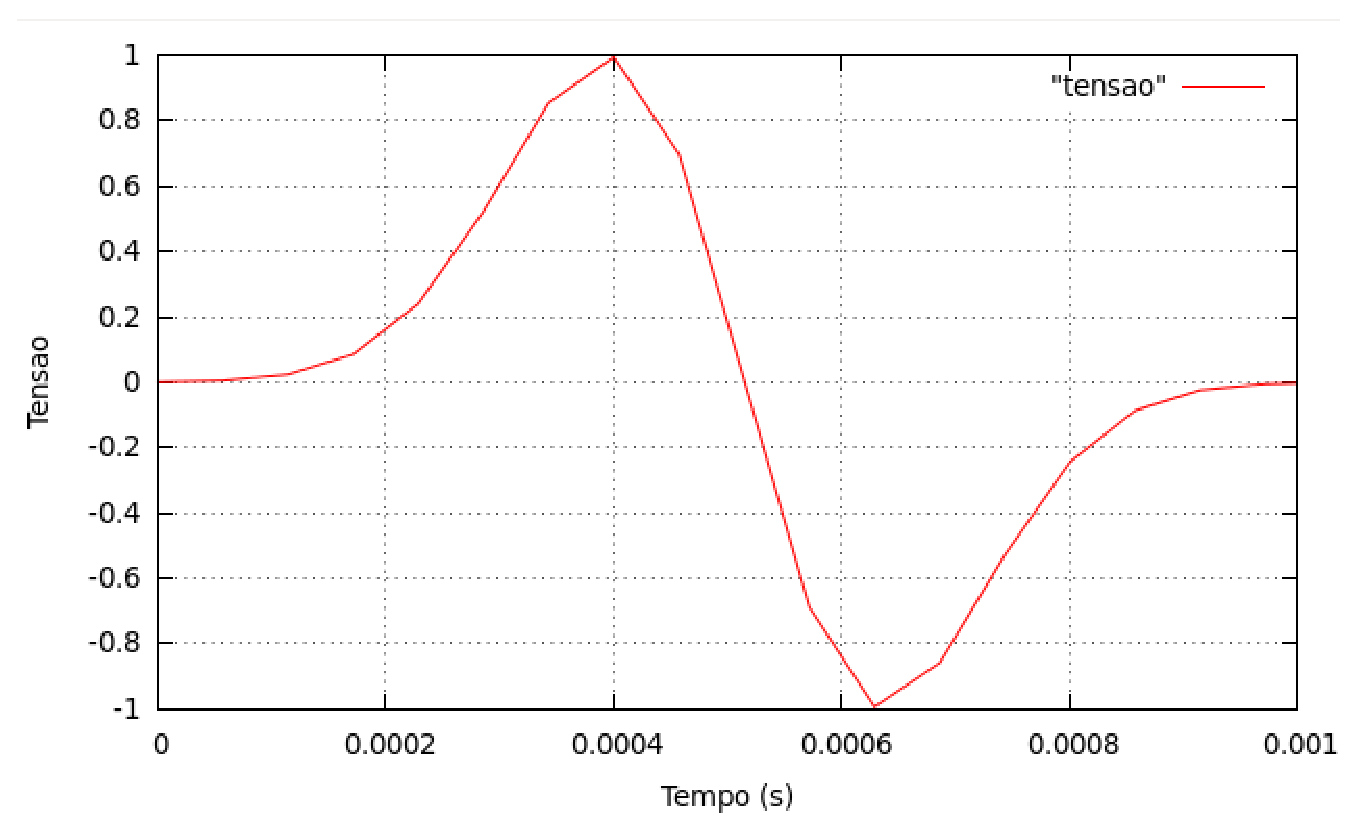
\includegraphics[scale = 0.4]{tensao}
%	\caption{Gráfico da fonte transformada de Fourier da fonte.}
%	\label{fg:fonte_f}
%\end{figure}

%\begin{figure}
%	\begin{subfigure}[b]{0.3\textwidth}
%			\centering
%			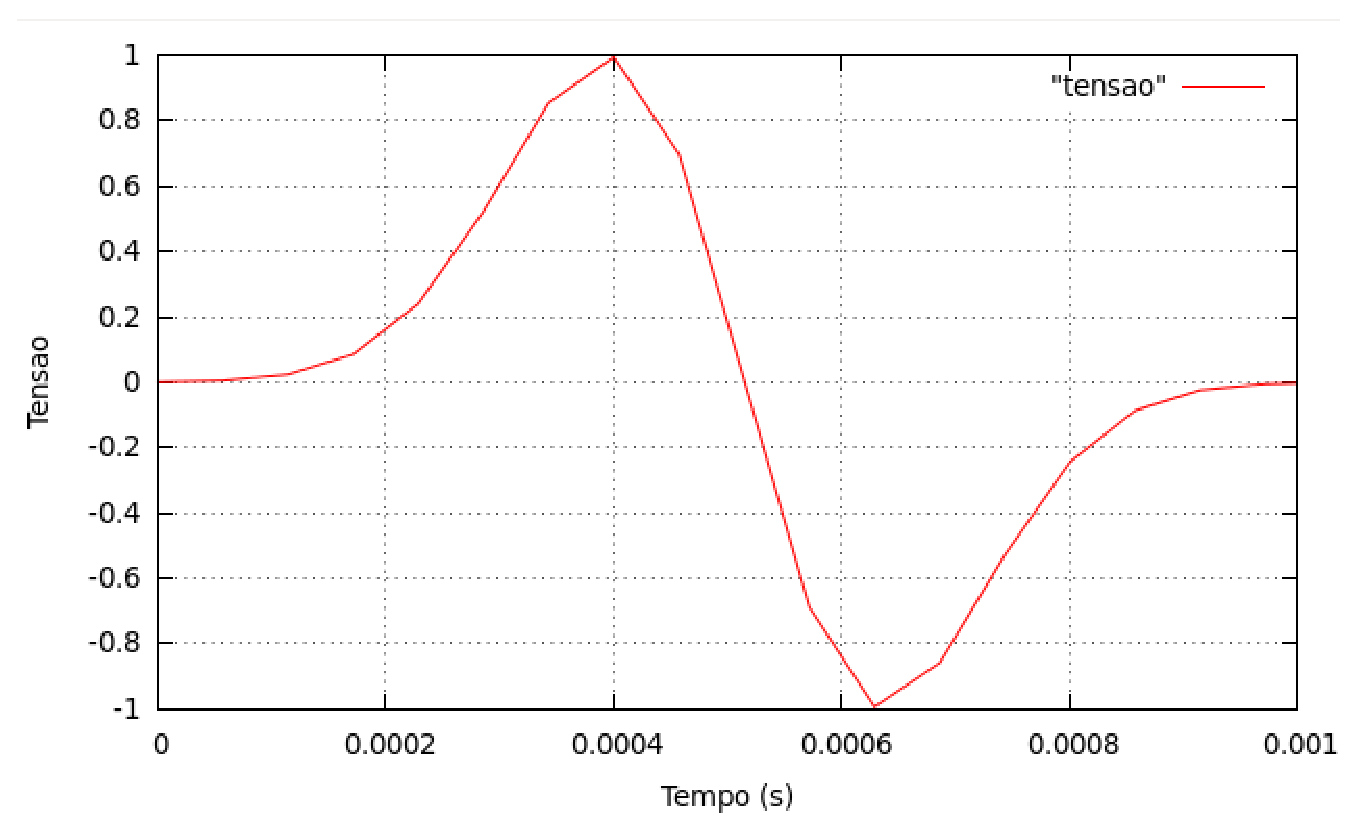
\includegraphics[width=\textwidth]{tensao}
%			\caption{Gráfico da fonte de tensão(trêm de pulsos).}
%			\label{fg:fonte}
%	\end{subfigure}%
%	~ %add desired spacing between images, e. g. ~, \quad, \qquad etc. 
%	  %(or a blank line to force the subfigure onto a new line)
%	\begin{subfigure}[b]{0.3\textwidth}
%			\centering
%			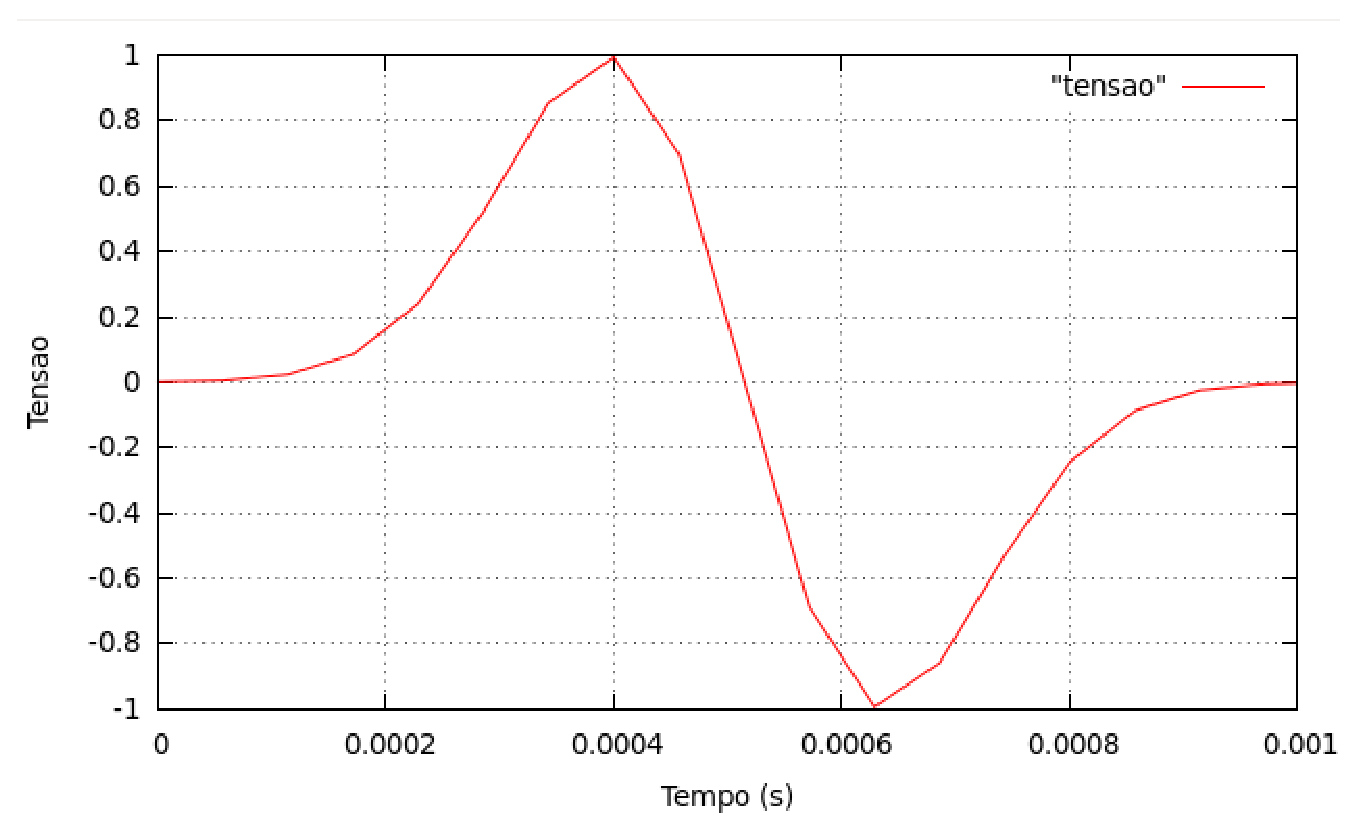
\includegraphics[width=\textwidth]{tensao}
%			\caption{Gráfico da transformada de Fourier da fonte (banda na qual esta trabalhando).}
%			\label{fg:fonte}
%	\end{subfigure}
%	~ %add desired spacing between images, e. g. ~, \quad, \qquad etc. 
%	  %(or a blank line to force the subfigure onto a new line)
%	\caption{Fonte da Antena}\label{fg:fonte_antena}
%\end{figure}





 Visto que o sua perda de retorno não foi satisfatória, foram feitas modificações em sua dimensão e por fim foi adicionado um  capacitor(Figura(colocar figura antena capacitor)). Com essas mudanças se obteve um antena com um comportamento parecido com o da real. Os gráficos de perda dessas duas construções esta ilustrado na Figura(colocar figura da perda)
%resultados
